\chapter{木のアルゴリズム - Tree algorithms}

\index{木}

\key{木} は、$n$個のノードと$n - 1$個のエッジからなる連結かつ閉路を含まないグラフです。
木から辺を1つ取り除くと2つの要素に分かれ、辺を加えると1つの閉路ができます。
また、木の任意の2つのノード間には常に一本のパスが存在します。

例えば、8個のノードと7個のエッジから構成されている木の例を示します。
\begin{center}
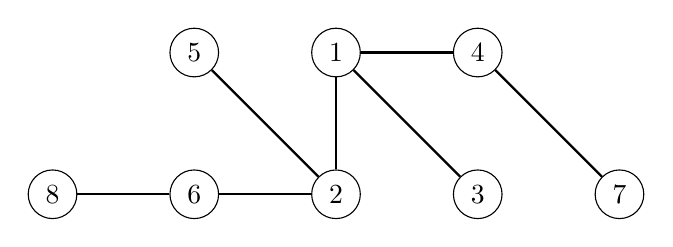
\begin{tikzpicture}[scale=0.9]
\node[draw, circle] (1) at (0,3) {$1$};
\node[draw, circle] (2) at (2,3) {$4$};
\node[draw, circle] (3) at (0,1) {$2$};
\node[draw, circle] (4) at (2,1) {$3$};
\node[draw, circle] (5) at (4,1) {$7$};
\node[draw, circle] (6) at (-2,3) {$5$};
\node[draw, circle] (7) at (-2,1) {$6$};
\node[draw, circle] (8) at (-4,1) {$8$};
\path[draw,thick,-] (1) -- (2);
\path[draw,thick,-] (1) -- (3);
\path[draw,thick,-] (1) -- (4);
\path[draw,thick,-] (2) -- (5);
\path[draw,thick,-] (3) -- (6);
\path[draw,thick,-] (3) -- (7);
\path[draw,thick,-] (7) -- (8);
\end{tikzpicture}
\end{center}

\index{leaf}

木の\key{葉}(リーフ)は、次数が1のノード、つまり、隣接ノードが1つしかないノードです。
上図の葉は、ノード$3,5,7,8$です。

\index{根}
\index{根付き木}

根付き木は、あるノードを木の根として指名し、
他のすべてのノードは 根の下に配置されます。
例えば、以下の木では、ノード1が根となるノード(ルートノード)です。

\begin{center}
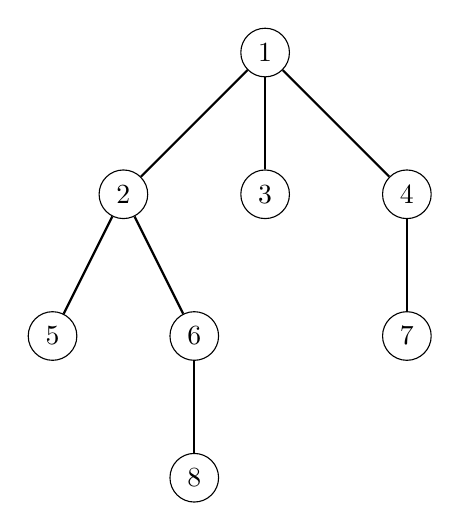
\begin{tikzpicture}[scale=0.9]
\node[draw, circle] (1) at (0,3) {$1$};
\node[draw, circle] (4) at (2,1) {$4$};
\node[draw, circle] (2) at (-2,1) {$2$};
\node[draw, circle] (3) at (0,1) {$3$};
\node[draw, circle] (7) at (2,-1) {$7$};
\node[draw, circle] (5) at (-3,-1) {$5$};
\node[draw, circle] (6) at (-1,-1) {$6$};
\node[draw, circle] (8) at (-1,-3) {$8$};
\path[draw,thick,-] (1) -- (2);
\path[draw,thick,-] (1) -- (3);
\path[draw,thick,-] (1) -- (4);
\path[draw,thick,-] (2) -- (5);
\path[draw,thick,-] (2) -- (6);
\path[draw,thick,-] (4) -- (7);
\path[draw,thick,-] (6) -- (8);
\end{tikzpicture}
\end{center}
\index{child}
\index{parent}

根付き木では、次の様に言葉を定義します。
\key{子}は配下にいる隣接ノード、\key{親}は上位の隣接ノードです。
根以外のノードは、ただ1つの親を持ちます。
上図の木では、ノード2の子はノード5とノード6です。ノード2の親はノード1です。

\index{部分木}

根付き木の構造は\emph{再帰的}です。
あるノードに注目した時にそのノードは、そのノード自身とそのノードの子の部分木に含まれるすべてのノードを含む部分木のルートとして機能します。
例えば、上図の木では、ノード2の部分木は、ノード2、5、6 、8です。

\begin{center}
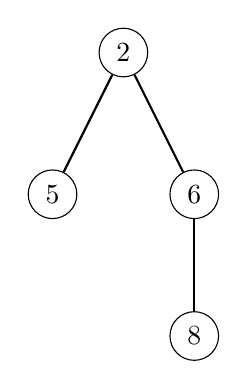
\begin{tikzpicture}[scale=0.9]
\node[draw, circle] (2) at (-2,1) {$2$};
\node[draw, circle] (5) at (-3,-1) {$5$};
\node[draw, circle] (6) at (-1,-1) {$6$};
\node[draw, circle] (8) at (-1,-3) {$8$};
\path[draw,thick,-] (2) -- (5);
\path[draw,thick,-] (2) -- (6);
\path[draw,thick,-] (6) -- (8);
\end{tikzpicture}
\end{center}

\section{木の探索 - Graph Traversal}

一般的なグラフの探索アルゴリズムは、木のノードを探索に使用することができます。
木には閉路がなく、親と子の関係で構成されているため木の探索は一般のグラフの探索よりも実装が簡単です。
最もシンプルな方法はあるノードから深さ優先探索します。次のような再帰的な関数が考えられます。

\begin{lstlisting}
void dfs(int s, int e) {
    // process node s
    for (auto u : adj[s]) {
        if (u != e) dfs(u, s);
    }
}
\end{lstlisting}

この関数は現在のノード$s$と直前のノード$e$が与えられます。
$e$はこれまでの訪問ノードの情報を持ちます。
この関数は次のように呼ぶとノード$x$から探索を開始します。

\begin{lstlisting}
dfs(x, 0);
\end{lstlisting}

$e=0$とすることで(訳註:この例ではノード0は存在しないので終わることはなく)最初のノードは全てのノードに移動できます。

\subsubsection{動的計画法 - Dynamic programming}

動的計画法は、木の探索中に何らかの情報を計算するために用いることができます。
根付き木において各ノードの部分木のノード数やそのノードから葉までの最長経路の長さといったものを$O(n)$時間で計算できます。

各ノード$s$について、その部分木に含まれるノードの数
$\texttt{count}[s]$求めてみましょう。
部分木には,ノード自身とその子の部分木に含まれるすべてのノードが含まれるので
以下のコードで再帰的にノード数を計算することができます。

\begin{lstlisting}
void dfs(int s, int e) {
    count[s] = 1;
    for (auto u : adj[s]) {
        if (u == e) continue;
        dfs(u, s);
        count[s] += count[u];
    }
}
\end{lstlisting}

\section{直径 - Diameter}

\index{直径}

木の\key{直径}とはその木に含まれる2ノード間の最長の距離です。
例を示します。

\begin{center}
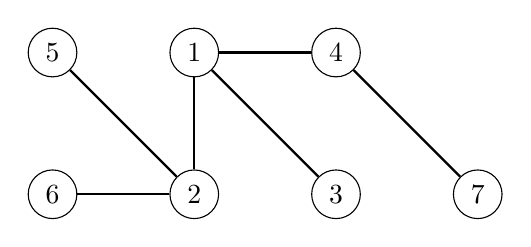
\begin{tikzpicture}[scale=0.9]
\node[draw, circle] (1) at (0,3) {$1$};
\node[draw, circle] (2) at (2,3) {$4$};
\node[draw, circle] (3) at (0,1) {$2$};
\node[draw, circle] (4) at (2,1) {$3$};
\node[draw, circle] (5) at (4,1) {$7$};
\node[draw, circle] (6) at (-2,3) {$5$};
\node[draw, circle] (7) at (-2,1) {$6$};
\path[draw,thick,-] (1) -- (2);
\path[draw,thick,-] (1) -- (3);
\path[draw,thick,-] (1) -- (4);
\path[draw,thick,-] (2) -- (5);
\path[draw,thick,-] (3) -- (6);
\path[draw,thick,-] (3) -- (7);
\end{tikzpicture}
\end{center}
この木の直径は次のパスの通り4です。
\begin{center}
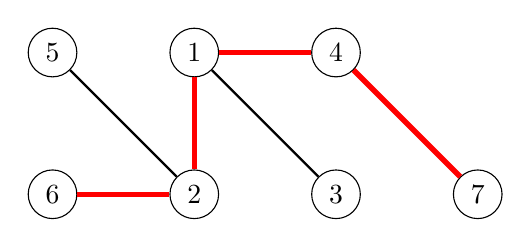
\begin{tikzpicture}[scale=0.9]
\node[draw, circle] (1) at (0,3) {$1$};
\node[draw, circle] (2) at (2,3) {$4$};
\node[draw, circle] (3) at (0,1) {$2$};
\node[draw, circle] (4) at (2,1) {$3$};
\node[draw, circle] (5) at (4,1) {$7$};
\node[draw, circle] (6) at (-2,3) {$5$};
\node[draw, circle] (7) at (-2,1) {$6$};
\path[draw,thick,-] (1) -- (2);
\path[draw,thick,-] (1) -- (3);
\path[draw,thick,-] (1) -- (4);
\path[draw,thick,-] (2) -- (5);
\path[draw,thick,-] (3) -- (6);
\path[draw,thick,-] (3) -- (7);

\path[draw,thick,-,color=red,line width=2pt] (7) -- (3);
\path[draw,thick,-,color=red,line width=2pt] (3) -- (1);
\path[draw,thick,-,color=red,line width=2pt] (1) -- (2);
\path[draw,thick,-,color=red,line width=2pt] (2) -- (5);
\end{tikzpicture}
\end{center}
半径の経路は複数存在する可能性があります。例えば上記の例ならノード6をノード5に置き換えると、
長さ4の別のパスを得ることができます。

木の直径を計算するための2つの$O(n)$のアルゴリズムを紹介します。
最初のアルゴリズムは動的計画法に基づいており、2番目のアルゴリズムは2つの深さ優先探索を用います。

\subsubsection{アルゴリズム1: 動的計画法}

木の問題を解く際によく使われるアプローチは木を根付き木と捉えることです。
この木を根付き木と捉える方法は部分木について個別に問題を解けば良いケースが多々あり、有効です。
このアルゴリズムはこのアプローチをとり、根付き木の各ノードにはそのパスを経由する最も長いパスが存在します。
各ノードについてそのノードに含まれる最長経路の長さを表せれば、そのパスの1つが木の直径に相当します。
例えば、以下の木では、ノード1が直径に相当する部分木のノードです。

\begin{center}
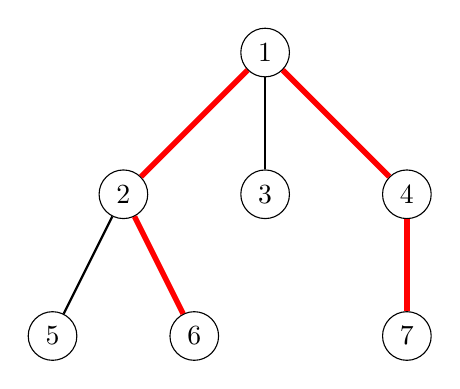
\begin{tikzpicture}[scale=0.9]
\node[draw, circle] (1) at (0,3) {$1$};
\node[draw, circle] (2) at (2,1) {$4$};
\node[draw, circle] (3) at (-2,1) {$2$};
\node[draw, circle] (4) at (0,1) {$3$};
\node[draw, circle] (5) at (2,-1) {$7$};
\node[draw, circle] (6) at (-3,-1) {$5$};
\node[draw, circle] (7) at (-1,-1) {$6$};
\path[draw,thick,-] (1) -- (2);
\path[draw,thick,-] (1) -- (3);
\path[draw,thick,-] (1) -- (4);
\path[draw,thick,-] (2) -- (5);
\path[draw,thick,-] (3) -- (6);
\path[draw,thick,-] (3) -- (7);

\path[draw,thick,-,color=red,line width=2pt] (7) -- (3);
\path[draw,thick,-,color=red,line width=2pt] (3) -- (1);
\path[draw,thick,-,color=red,line width=2pt] (1) -- (2);
\path[draw,thick,-,color=red,line width=2pt] (2) -- (5);
\end{tikzpicture}
\end{center}


各ノード$x$に対して以下の2つを求めます。
\begin{itemize}
\item $\texttt{toLeaf}(x)$: $x$から葉まで最大長
\item $\texttt{maxLength}(x)$: 最高点が$x$であるパスの最大長
\end{itemize}

例えば上の図の木では
$1 \rightarrow 2 \rightarrow 6$があるため
$\texttt{toLeaf}(1)=2$となり、
$6 \rightarrow 2 \rightarrow 1 \rightarrow 4 \rightarrow 7$があるので
$\texttt{maxLength}(1)=4$となります。
この例では $\texttt{maxLength}(1)$が直径となります。

動的計画法を用いて上記の値を全ノードについて$O(n)$時間で計算することができます。
まず、$\texttt{toLeaf}(x)$を計算するために、$x$の子ノードを調べ、
$\texttt{toLeaf}(c)$が最大である子$c$を選んで、この値に1を足します。
次に、$\texttt{maxLength}(x)$を計算するために、
$\texttt{toLeaf}(a)+\texttt{toLeaf}(b)$の和が最大となるような異なる二つの子 $a$ と $b$ を選び、
この和に2を足します。
(訳註:このような計算は木DPとも呼ばれます)

\subsubsection{アルゴリズム2: 深さ優先探索}

木の直径を計算するためにもう一つの効率的な方法を紹介します。
2回の深さ優先探索を利用した方法です。
まず、木の任意のノード$a$を選び、$a$から最も遠いノード$b$を見つけます。
$b$から最も遠いノード$c$を見つけます。木の直径は$b$と$c$の間の距離となります。
次のグラフで$a$,$b$,$c$を次のように置くことができます。

\begin{center}
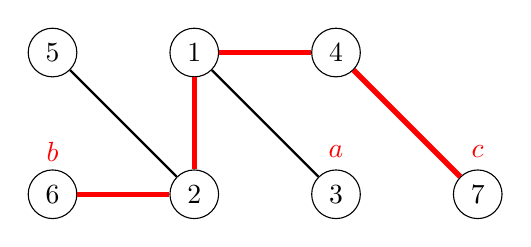
\begin{tikzpicture}[scale=0.9]
\node[draw, circle] (1) at (0,3) {$1$};
\node[draw, circle] (2) at (2,3) {$4$};
\node[draw, circle] (3) at (0,1) {$2$};
\node[draw, circle] (4) at (2,1) {$3$};
\node[draw, circle] (5) at (4,1) {$7$};
\node[draw, circle] (6) at (-2,3) {$5$};
\node[draw, circle] (7) at (-2,1) {$6$};
\path[draw,thick,-] (1) -- (2);
\path[draw,thick,-] (1) -- (3);
\path[draw,thick,-] (1) -- (4);
\path[draw,thick,-] (2) -- (5);
\path[draw,thick,-] (3) -- (6);
\path[draw,thick,-] (3) -- (7);
\node[color=red] at (2,1.6) {$a$};
\node[color=red] at (-2,1.6) {$b$};
\node[color=red] at (4,1.6) {$c$};

\path[draw,thick,-,color=red,line width=2pt] (7) -- (3);
\path[draw,thick,-,color=red,line width=2pt] (3) -- (1);
\path[draw,thick,-,color=red,line width=2pt] (1) -- (2);
\path[draw,thick,-,color=red,line width=2pt] (2) -- (5);
\end{tikzpicture}
\end{center}

たったこれだけです。本当にうまく動作するのでしょうか?
ツリーの向きを変えて直径のパスが水平になるように表現します。
\begin{center}
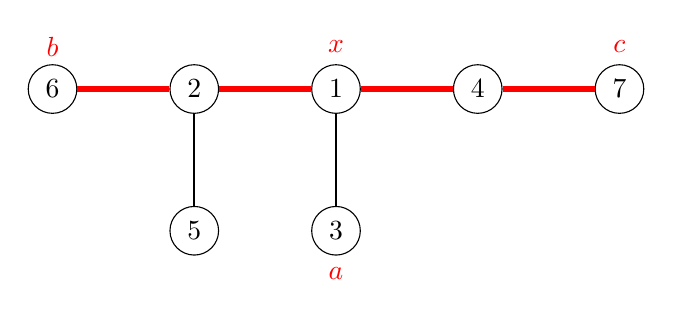
\begin{tikzpicture}[scale=0.9]
\node[draw, circle] (1) at (2,1) {$1$};
\node[draw, circle] (2) at (4,1) {$4$};
\node[draw, circle] (3) at (0,1) {$2$};
\node[draw, circle] (4) at (2,-1) {$3$};
\node[draw, circle] (5) at (6,1) {$7$};
\node[draw, circle] (6) at (0,-1) {$5$};
\node[draw, circle] (7) at (-2,1) {$6$};
\path[draw,thick,-] (1) -- (2);
\path[draw,thick,-] (1) -- (3);
\path[draw,thick,-] (1) -- (4);
\path[draw,thick,-] (2) -- (5);
\path[draw,thick,-] (3) -- (6);
\path[draw,thick,-] (3) -- (7);
\node[color=red] at (2,-1.6) {$a$};
\node[color=red] at (-2,1.6) {$b$};
\node[color=red] at (6,1.6) {$c$};
\node[color=red] at (2,1.6) {$x$};

\path[draw,thick,-,color=red,line width=2pt] (7) -- (3);
\path[draw,thick,-,color=red,line width=2pt] (3) -- (1);
\path[draw,thick,-,color=red,line width=2pt] (1) -- (2);
\path[draw,thick,-,color=red,line width=2pt] (2) -- (5);
\end{tikzpicture}
\end{center}

ノード$x$は、ノード$a$からの経路が直径に対応する経路に合流するノードとしましょう。
$a$から最も遠いノードは$b$とはノード $c$あるいはノード$x$から少なくとも同じだけ遠い異なるノードです。
したがって、このノードは直径に対応するパスの終点として常に有効な候補となります。
(訳注: $a$から辿るとこの表現をした際の水平の線に必ず合流します。
なので1回目のBFSでそこから最も遠い距離を探すことはいずれかの水平な線の候補の端点を見つけることとなり、そこからBFSを再度行えば同じ様にもう一方の端点を探せます)

\section{全ノードからの最長経路 - All longest paths}


木の各ノードについて、
そのノードから始まる最大の経路の長さを計算することを考えましょう。
これは木の直径問題の一般化とも言えます。
それらの長さのうち最大のものは木の直径だからです。

この問題は$O(n)$で解くことができます。
\begin{center}
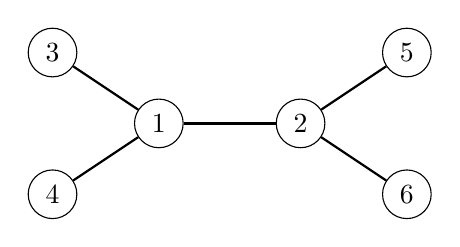
\begin{tikzpicture}[scale=0.9]
\node[draw, circle] (1) at (0,0) {$1$};
\node[draw, circle] (2) at (-1.5,-1) {$4$};
\node[draw, circle] (3) at (2,0) {$2$};
\node[draw, circle] (4) at (-1.5,1) {$3$};
\node[draw, circle] (6) at (3.5,-1) {$6$};
\node[draw, circle] (7) at (3.5,1) {$5$};
\path[draw,thick,-] (1) -- (2);
\path[draw,thick,-] (1) -- (3);
\path[draw,thick,-] (1) -- (4);
\path[draw,thick,-] (3) -- (6);
\path[draw,thick,-] (3) -- (7);
\end{tikzpicture}
\end{center}

$\texttt{maxLength}(x)$を$x$を始点とするパスの最大長とします。
上図の木では
$\rightarrow 1 \rightarrow 2 \rightarrow 6$
というパスがあるので、
$\texttt{maxLength}(4)=3$です。これを表にします。
\begin{center}
\begin{tabular}{l|lllllll}
ノード$x$ & 1 & 2 & 3 & 4 & 5 & 6 \\
$\texttt{maxLength}(x)$ & 2 & 2 & 3 & 3 & 3 & 3 \\
\end{tabular}
\end{center}

先ほどと同じ様に根付き木にすると見通しがよくなります。
\begin{center}
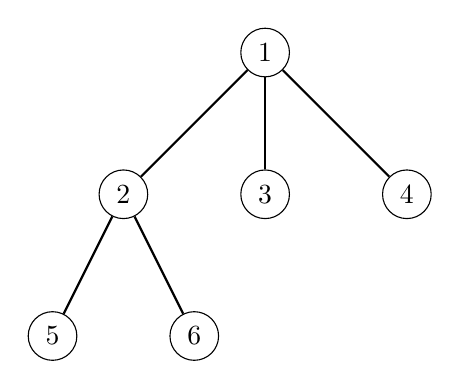
\begin{tikzpicture}[scale=0.9]
\node[draw, circle] (1) at (0,3) {$1$};
\node[draw, circle] (2) at (2,1) {$4$};
\node[draw, circle] (3) at (-2,1) {$2$};
\node[draw, circle] (4) at (0,1) {$3$};
\node[draw, circle] (6) at (-3,-1) {$5$};
\node[draw, circle] (7) at (-1,-1) {$6$};
\path[draw,thick,-] (1) -- (2);
\path[draw,thick,-] (1) -- (3);
\path[draw,thick,-] (1) -- (4);
\path[draw,thick,-] (3) -- (6);
\path[draw,thick,-] (3) -- (7);
\end{tikzpicture}
\end{center}

各$x$について、その子のノードの中で最長のパスを持つノードを探します。
例えば、ノード1からの最長の経路はその子2を通ることがわかります。

\begin{center}
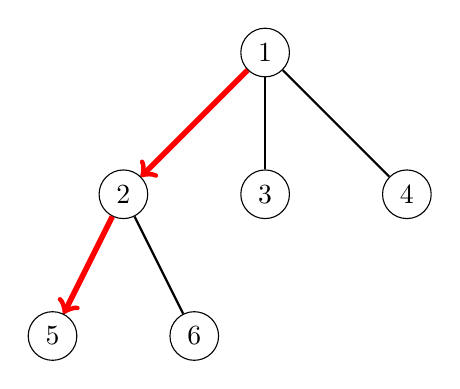
\begin{tikzpicture}[scale=0.9]
\node[draw, circle] (1) at (0,3) {$1$};
\node[draw, circle] (2) at (2,1) {$4$};
\node[draw, circle] (3) at (-2,1) {$2$};
\node[draw, circle] (4) at (0,1) {$3$};
\node[draw, circle] (6) at (-3,-1) {$5$};
\node[draw, circle] (7) at (-1,-1) {$6$};
\path[draw,thick,-] (1) -- (2);
\path[draw,thick,-] (1) -- (3);
\path[draw,thick,-] (1) -- (4);
\path[draw,thick,-] (3) -- (6);
\path[draw,thick,-] (3) -- (7);

\path[draw,thick,->,color=red,line width=2pt] (1) -- (3);
\path[draw,thick,->,color=red,line width=2pt] (3) -- (6);
\end{tikzpicture}
\end{center}

これは前回と同様に動的計画法で$O(n)$で解くことができます。
例えば、ノード3からの最長経路はその親1を通る。

次に、各ノードに対して、以下の計算を行います。
各ノード $x$ について、親 $p$ を通る経路の最大長を計算します。
例えば、ノード3からの最長経路はその親1を通ります。

\begin{center}
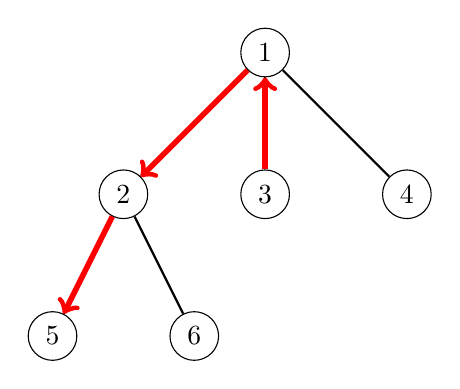
\begin{tikzpicture}[scale=0.9]
\node[draw, circle] (1) at (0,3) {$1$};
\node[draw, circle] (2) at (2,1) {$4$};
\node[draw, circle] (3) at (-2,1) {$2$};
\node[draw, circle] (4) at (0,1) {$3$};
\node[draw, circle] (6) at (-3,-1) {$5$};
\node[draw, circle] (7) at (-1,-1) {$6$};
\path[draw,thick,-] (1) -- (2);
\path[draw,thick,-] (1) -- (3);
\path[draw,thick,-] (1) -- (4);
\path[draw,thick,-] (3) -- (6);
\path[draw,thick,-] (3) -- (7);

\path[draw,thick,->,color=red,line width=2pt] (4) -- (1);
\path[draw,thick,->,color=red,line width=2pt] (1) -- (3);
\path[draw,thick,->,color=red,line width=2pt] (3) -- (6);
\end{tikzpicture}
\end{center}

これは$p$からの最長経路を選べばよさそうにみえますが、
$p$からの最長経路が$x$を経由する場合があるため、
必ずしもうまくいかきません。
次の様な例があります。

\begin{center}
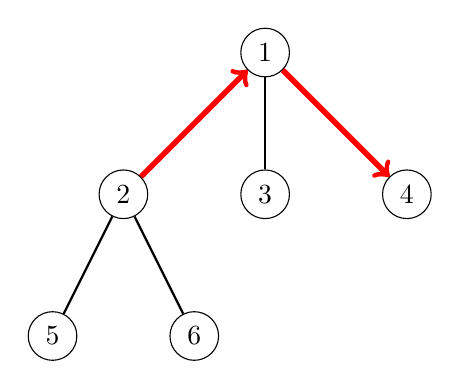
\begin{tikzpicture}[scale=0.9]
\node[draw, circle] (1) at (0,3) {$1$};
\node[draw, circle] (2) at (2,1) {$4$};
\node[draw, circle] (3) at (-2,1) {$2$};
\node[draw, circle] (4) at (0,1) {$3$};
\node[draw, circle] (6) at (-3,-1) {$5$};
\node[draw, circle] (7) at (-1,-1) {$6$};
\path[draw,thick,-] (1) -- (2);
\path[draw,thick,-] (1) -- (3);
\path[draw,thick,-] (1) -- (4);
\path[draw,thick,-] (3) -- (6);
\path[draw,thick,-] (3) -- (7);

\path[draw,thick,->,color=red,line width=2pt] (3) -- (1);
\path[draw,thick,->,color=red,line width=2pt] (1) -- (2);
\end{tikzpicture}
\end{center}

ですが、各ノード$x$について2つの最大長を記憶することで、$O(n)$で解くことができます。まずは次の2つを定義しましょう。
\begin{itemize}
\item $\texttt{maxLength}_1(x)$:
$x$からの最大のパス長
\item $\texttt{maxLength}_2(x)$
それとは異なる次の最大のパス長。長さは同じこともある。
\end{itemize}

上記のグラフでは
$1 \rightarrow 2 \rightarrow 5$から
$\texttt{maxLength}_1(1)=2$
であり、
$1 \rightarrow 3$から
$\texttt{maxLength}_2(1)=1$となります。

$\texttt{maxLength}_1(p)$に対応するパスが$x$を通る時、
$\texttt{maxLength}_2(p)+1$ということができます。
そうでない場合は、$\texttt{maxLength}_1(p)+1$となります。

\section{二分木 - Binary trees}

\index{二分木 - binary tree}

\begin{samepage}

\key{二分木}とは、
全てのノードが左と右に部分木を持つ根付きの木のことである。
ただし、部分木が空であることも許容します。
言い換えれば、二分木のすべてのノードは$0$個、$1$個、または$2$個の子を持つと言えます。

例を示します。
\begin{center}
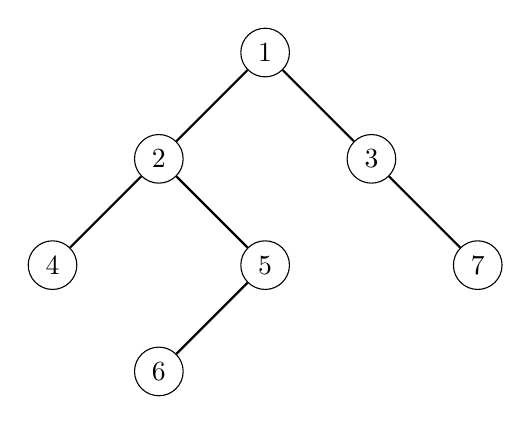
\begin{tikzpicture}[scale=0.9]
\node[draw, circle] (1) at (0,0) {$1$};
\node[draw, circle] (2) at (-1.5,-1.5) {$2$};
\node[draw, circle] (3) at (1.5,-1.5) {$3$};
\node[draw, circle] (4) at (-3,-3) {$4$};
\node[draw, circle] (5) at (0,-3) {$5$};
\node[draw, circle] (6) at (-1.5,-4.5) {$6$};
\node[draw, circle] (7) at (3,-3) {$7$};

\path[draw,thick,-] (1) -- (2);
\path[draw,thick,-] (1) -- (3);
\path[draw,thick,-] (2) -- (4);
\path[draw,thick,-] (2) -- (5);
\path[draw,thick,-] (5) -- (6);
\path[draw,thick,-] (3) -- (7);
\end{tikzpicture}
\end{center}
\end{samepage}

\index{pre-order}
\index{in-order}
\index{post-order}
二分木のノードには3つの自然な走査(Traversal)があります。
\begin{itemize}
\item \key{pre-order}: ルートを処理してから左を処理する。次に右を処理する。
\item \key{in-order}: 左を処理してからルートを処理する。次に右を処理する。
\item \key{post-order}: 左を処理してから右を処理する。次にルートを処理する。
\end{itemize}

上記の木では、
pre-orderは$[1,2,4,5,6,3,7]$,
in-orderは$[4,2,6,5,1,3,7]$,
post-orderは$[4,6,5,2,7,3,1]$となります。

また、pre-orderとin-orderの2つが分かると木が復元できることも知られています。
例えば、pre-order$[1,2,4,5,6,3,7]$でin-order$[4,2,6,5,1,3,7]$とわかれば上の木を復元できます。
同様にpost-orderとin-orderがわかっている場合も復元できます。

ただし、pre-orderとpost-orderだけがわかっている場合は注意が必要です。
条件を満たす複数の可能性があるからです。この例をみてみます。
\begin{center}
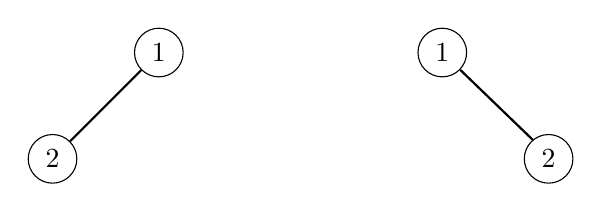
\begin{tikzpicture}[scale=0.9]
\node[draw, circle] (1) at (0,0) {$1$};
\node[draw, circle] (2) at (-1.5,-1.5) {$2$};
\path[draw,thick,-] (1) -- (2);

\node[draw, circle] (1b) at (0+4,0) {$1$};
\node[draw, circle] (2b) at (1.5+4,-1.5) {$2$};
\path[draw,thick,-] (1b) -- (2b);
\end{tikzpicture}
\end{center}
どちらの木も pre-order $[1,2]$ で post-order is $[2,1]$です。このため、どちらかに確定させることはできません。
